%\index{\footnote{}}
\chapter{Introduction}%\label{Introduction}

Small paragraph to make reader interested in further reading. 

\section{Background}

Write background of your project.
%Background, problem statement, available solutions (if any),your solution with justification, timeplan.

\section{Problem Statement}

\subsection{Objectives and Scope}

\subsubsection{Objectives}
\paragraph{}
gfugfsghdgdshgfdh dahba 
\begin{itemize}
	\item Objective 1
	\item Objective 2
	\item ..
\end{itemize}

\subsubsection{Scope}
\begin{itemize}
	\item Scope 1
	\paragraph{}
	asdajskbgsvdhfbgsdhbf
	\item Scope 2
	\item ..
\end{itemize}

\subsection{Research Methodology}
\subsubsection{Example for add image}

\begin{figure}[H]
	\begin{center}
		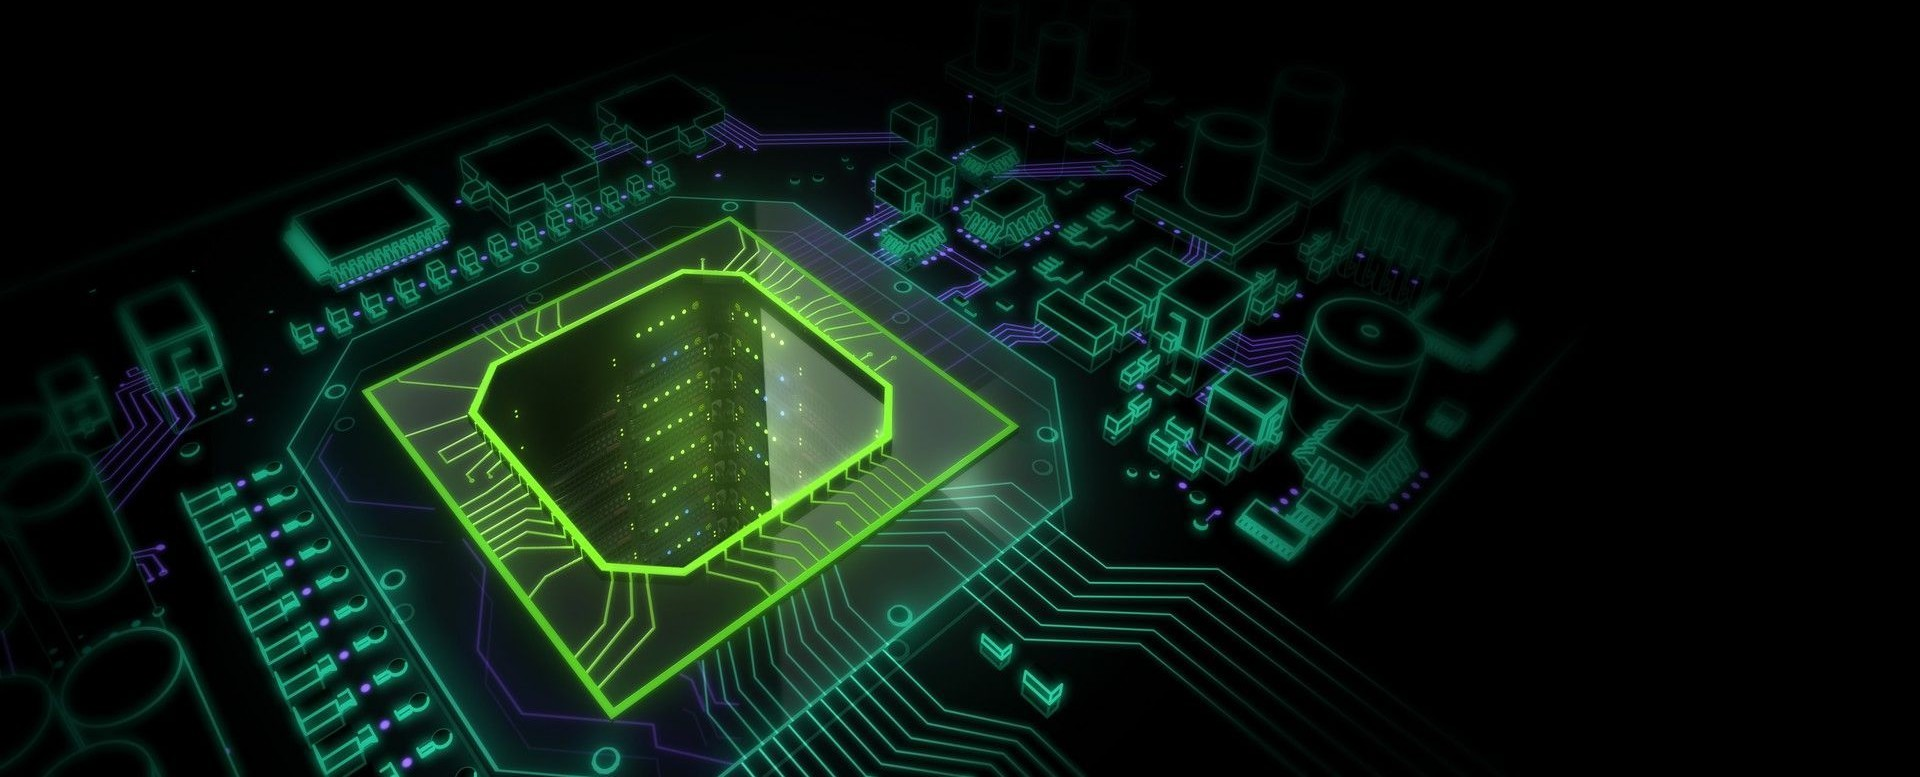
\includegraphics[width=0.9\textwidth]{01_chapters/01/figs/exsample.jpg}
	\end{center}
	\caption{Image Caption}
\end{figure}

\begin{table}[tb]
	\caption{\textbf{table caption}}
	\label{tb:sampletable}
	
	\begin{center}
		
		\begin{tabular}{|c|c|c|c|}
			\hline \textbf{Col 1} & \textbf{Col 2} & \textbf{Col 3} & \textbf{Col4}    \\
			
			\hline  data 1        & data 2         & data 3         & data 4           \\ 
			\hline  data 1        & data 2         & data 3         & data 4           \\ 
			\hline  data 1        & data 2         & data 3         & data 4           \\ 
			
			\hline 
		\end{tabular} 
		
	\end{center}
\end{table}


\section{Time Plan and Required Resources}



%%%%%%%%%%%%%%%%%%%%%%%%%%%%%%%%%%%%%%%%%%%%%%%%%%%%%%%%%%%%%%%%%%%%%%%%%%%%%%%%%%%%%%%%%%%%%%%%%%
%%%%%%%%%%% END OF FILE
%%%%%%%%%%%%%%%%%%%%%%%%%%%%%%%%%%%%%%%%%%%%%%%%%%%%%%%%%%%%%%%%%%%%%%%%%%%%%%%%%%%%%%%%%%%%%%%%%%
